\documentclass[10pt,a4paper]{article}
\usepackage[margin=2.2cm]{geometry}
\usepackage{fontspec}
\usepackage{kotex}
\setmainfont{Apple SD Gothic Neo}
\setsansfont{Apple SD Gothic Neo}
\usepackage{amsmath,amssymb}
\usepackage{graphicx}
\usepackage{booktabs}
\usepackage{caption}
\usepackage[dvipsnames]{xcolor}
\usepackage[colorlinks=true,linkcolor=MidnightBlue,citecolor=MidnightBlue,
            urlcolor=MidnightBlue]{hyperref}
\usepackage{titlesec}
\titleformat{\section}{\large\bfseries}{\thesection}{0.6em}{}
\titleformat{\subsection}{\normalsize\bfseries}{\thesubsection}{0.5em}{}
\captionsetup{font=small,labelfont=bf}
\setlength{\parskip}{0.35em}
\setlength{\parindent}{0pt}

\usepackage{mdframed}
\newmdenv[linewidth=0.4pt,linecolor=gray!60,backgroundcolor=gray!5,
          innertopmargin=6pt,innerbottommargin=6pt,skipabove=8pt,skipbelow=8pt]{claimbox}
\newcommand{\claim}[2]{\begin{claimbox}\textbf{주장.} #1\par\smallskip
  \textcolor{gray!70}{\textbf{반증 조건.} #2}\end{claimbox}}

\title{\bfseries 장부에만 있던 고침\\[2pt]
\large 그리고 그것이 설명하지 못한 것}
\author{월드모델 실험실 · 노트 670}
\date{2026-08-06}
\begin{document}\maketitle

\section{한 줄}

대장에 ``돌리기 전에 코드를 읽다가 결함을 잡아 고쳤다''고 적혀 있었다. \textbf{그
고침은 git 이력에 한 번도 없었다.} 뒤따른 두 노트가 결함이 있는 축을 쟀다. 고쳐서
다시 재니 결함은 실재했고 --- 그런데 \textbf{내가 그 결함 탓으로 돌린 관측은
고친 뒤에도 그대로 남았다}.

\section{어떻게 찾았나}

노트 668 의 판 측정이 CPU 를 다 쓰는 동안 \emph{읽기만 하는 일}을 골랐다: 축
모듈들이 노트 645 규칙(정규화 통계도 누출)을 지키나 훑는 것. 그러다
\verb|lab/crowdaxes.py:121| 에서 이것을 봤다.

\begin{center}
\verb|same = sum(1 for k in range(j0, j1) if pool[k][1] & g)|
\end{center}

갈래 \textbf{합집합} 매칭이다. \emph{갈래를 하나라도 공유하는} 이전 출시를 세므로
갈래를 많이 단 작품이 기계적으로 높은 값을 받는다. 그런데 이 문장은 노트 650 대장에
\textbf{이미 적혀 있었다} --- ``이 결함을 잡아서 갈래 각각의 몫을 평균하도록 고쳤고
누적합으로 만들었다''고. \verb|git log --all -p| 에 \verb|cumsum| 이 \textbf{0회}이고
파일은 커밋 한 번으로 추가된 뒤 안 바뀌었다.

\claim{노트 546·549 의 조항 \emph{`장부와 코드가 따로 자란다'} 의 세 번째 자리다.
앞의 둘(provenance 미등록 · 축 등록 누락)은 \textbf{감사가 잡을 수 있는 모양}이었다.
이번은 아니다 --- \textbf{고침 자체가 장부에만 있었고}, 감사는 ``무엇이 등록됐나''를
보지 ``적어 둔 고침이 코드에 있나''를 보지 않는다.}
{같은 저장소에서 대장이 주장하는 코드 변경과 실제 diff 를 대조해 불일치가
없으면 이 주장은 일회성 사고다. 다만 조항이 두 번 먼저 발동했으므로 일회성으로
취급하지 않는다.}

\section{쟀다 --- 판을 안 돌고}

두 버전(합집합 · 갈래별 평균)을 나란히 만들고 \textbf{학습 행만}으로 넷을 쟀다.
유보는 안 본다(노트 568). 판을 안 도는 이유는 사전등록에 적었다 --- 결정 규칙이
``고친 축이 창에 민감해지면 판을 돈다''였다.

\begin{figure}[t]\centering
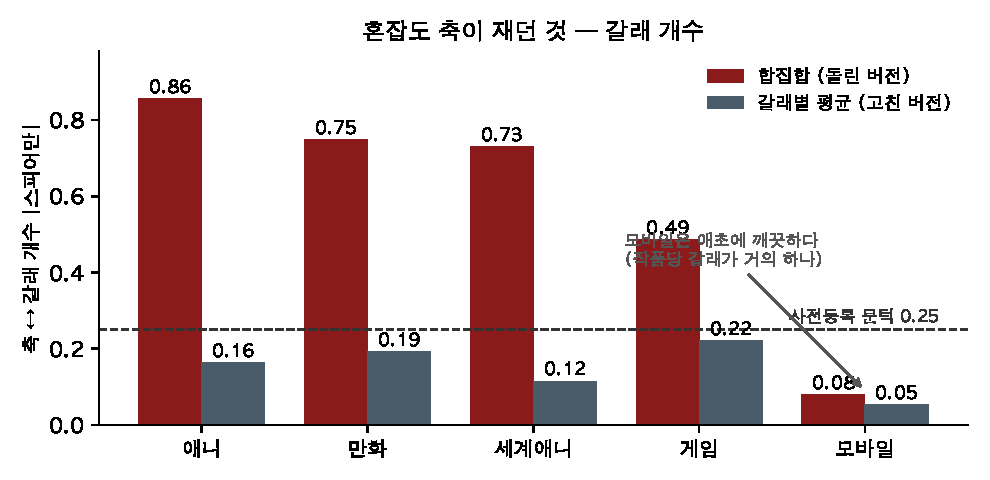
\includegraphics[width=0.9\textwidth]{figs/killed.pdf}
\caption{결함은 실재했다. 합집합 축은 애니 $0.856$ · 만화 $0.749$ · 세계애니
$0.730$ 으로 \textbf{갈래 개수와 강하게 붙는다}. 고치면 다섯 도메인 전부 사전등록
문턱 $0.25$ 아래로 내려간다. 게임은 $0.486$ 으로 문턱 $0.5$ 바로 아래고,
모바일은 애초에 깨끗했다 --- 작품당 갈래가 거의 하나라 두 정의가 같은 값이 된다.}
\end{figure}

축 $\leftrightarrow$ 라벨 |스피어만|(학습 · 가중 · 창 90일)은
$\mathbf{0.1462 \to 0.1051}$ 이다. 노트 650·651 이 본 $|r| \approx 0.13$ 의
\textbf{28\%가 갈래 개수 몫}이었다.

\section{그런데 내 예측이 틀렸다}

사전등록에 이렇게 적었다 --- \emph{``갈래 개수는 작품의 상수이므로 창을 12배 바꿔도
안 변한다. 노트 651 이 관측한 창 불변과 자기상관 $0.87\sim0.91$ 이 정확히 그
지문이다. 고치면 값이 창에 따라 실제로 달라질 것으로 본다.''}

\begin{figure}[t]\centering
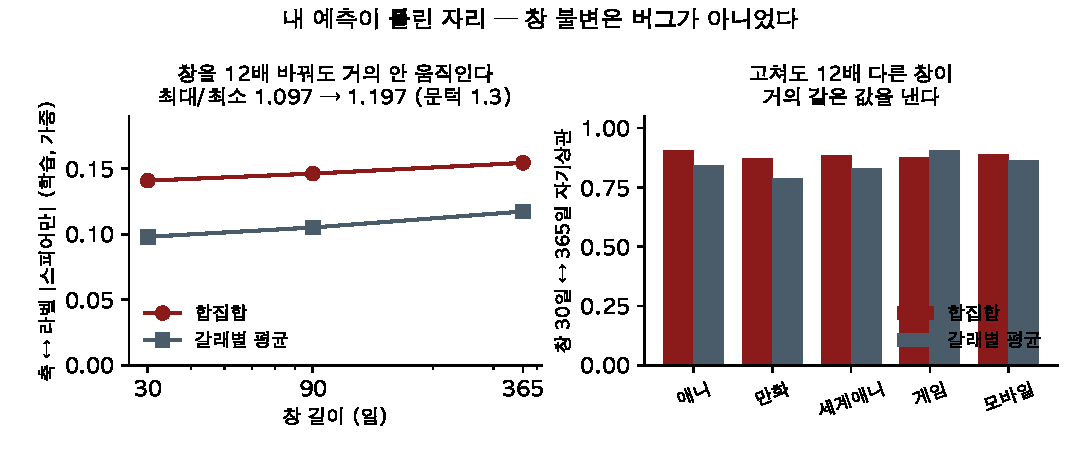
\includegraphics[width=0.98\textwidth]{figs/survived.pdf}
\caption{고친 축의 창 최대/최소는 $1.097 \to \mathbf{1.197}$ 로 조금 올랐지만
문턱 $1.3$ 을 못 넘는다. 창 30일 $\leftrightarrow$ 365일 자기상관도 여전히 높다
(게임 $0.905$ · 모바일 $0.862$ · 세계애니 $0.829$ · 애니 $0.843$ · 만화 $0.789$).
\textbf{갈래 개수를 뺀 뒤에도 12배 다른 창이 거의 같은 값을 낸다.}}
\end{figure}

\claim{\textbf{창 불변은 버그가 아니었다.} 노트 651 의 결론 --- 축이 최근 혼잡이
아니라 \emph{느리게 변하는 갈래 구성 수준}을 잰다 --- 은 고친 축에서 재현된다.
결함은 그 관측의 \textbf{크기}를 부풀렸지만 \textbf{원인은 아니었다}.}
{고친 축의 창 최대/최소가 $1.3$ 을 넘게 측정되면 이 주장은 뒤집힌다. 지금
$1.197$ 이라 문턱에 가깝다 --- 창을 더 촘촘히(15·45·180·730일) 재면 넘을 수 있다.
그것이 이 주장의 제일 약한 자리다.}

\section{그래서 두 노트를 어떻게 다시 읽나}

\begin{itemize}
\item \textbf{노트 651 의 결론은 산다.} 판정 근거가 고친 축에서도 재현된다.
\item \textbf{노트 650 의 숫자는 버그 판이다.} 신호 몫 $+0.0021$(``상태 축 최초로
      위약을 이김'')은 갈래 개수가 28\% 섞인 축의 값이다. \textbf{고친 축의 판
      효과는 안 재 봤다.}
\item 그래서 \textbf{(시간 $\times$ 대상) 규칙은 아직 제대로 시험되지 않았다.}
      노트 650·651 은 결함 있는 축을 쟀고, 노트 659 의 뉴스 축은 구글이
      500요청에서 막아 427행에서 멈췄다. \textbf{규칙을 반증된 것으로 취급하지
      않는다} --- 시험이 없었을 뿐이다.
\end{itemize}

판을 다시 도는 것은 값이 낮다. 상관이 28\% 줄었으므로 노트 650 의 $+0.0021$ 은
$+0.0015$ 안팎이 되고 문턱 $0.0045$ 에서 더 멀어진다. 돌리는 조건은 하나 ---
\textbf{이 축을 다른 형태로 다시 지을 때}(갈래 구성의 \emph{수준}이 아니라
\emph{변화}를 쓰는 축) 기준선으로 한 번 잰다.

\section{규약을 하나 더 만든다}

\begin{center}
\textbf{대장에 ``고쳤다''를 적으려면 그 고침이 같은 커밋에 있어야 한다.}
\end{center}

이번에 그렇게 했다 --- 고침을 코드에 넣고 커밋한 다음 이 결과를 적었다. 그리고
이 논문에서 제일 값이 큰 문장은 결함을 찾은 것이 아니라 \textbf{결함이 설명하지
못한 것을 찾은 것}이다. 버그를 찾으면 그 버그로 앞선 관측을 다 설명하고 싶어진다.
이번에는 \textbf{절반만} 설명했다.

\end{document}
